%!TEX program = xelatex
%!TEX encoding = UTF-8 Unicode

\documentclass[14pt, AutoFakeBold]{ldr}
  

\title{本 科 生 毕 业 答 辩}
\subtitle{利用机器学习进行气体探测器径迹重建的算法研究}

\author{答辩人:王文军}
\institute{指导老师:张毅}
\date{\today}
\titlegraphic{
\includegraphics[height=0.15\textwidth]{lzu_logo.png}}



  



\begin{document}

\maketitle

\AtBeginSection[]
{
  \begin{frame}
    \frametitle{\insertshorttitle}
    \tableofcontents[currentsection,hideallsubsections]
  \end{frame}
}





\section{研究背景}
\subsection{基于裂变时间投影室的新型核裂变测量技术}
\begin{frame}[c]{基于裂变时间投影室的新型核裂变测量技术}
利用机器学习进行\textcolor{red}{气体探测器径迹重建}的算法研究


  \frametitle{基于裂变时间投影室的新型核裂变测量技术}
  \begin{figure}[H]
  \centering
  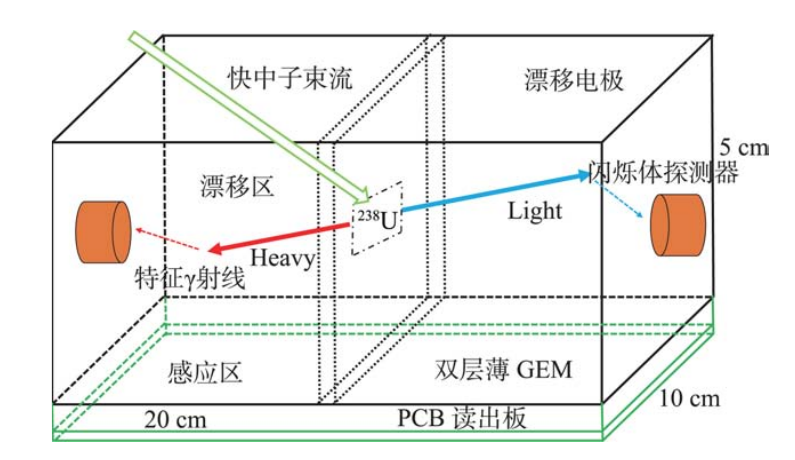
\includegraphics[width=0.9\textwidth]{../figures/GEM-TPC.png}

  \caption{裂变时间投影室探测系统(论文 P6)}
  \label{fig-GEM-TPC}
  \end{figure}
  
\end{frame}



\begin{frame}
  \frametitle{时间投影室的应用}
  \begin{itemize}
    \item 许多大型高能粒子实验都采用其作为中心径迹探测器, 比较著名的有LEP实验的ALEPH, DELPHI, BNL的 STAR, LHC的ALICE等等。
    \item MicroBooNE Collaboration 应用卷积神经网络完成了对时间投影室产生的径迹数据的算法研究。算法包括多粒子径迹图片的分类(Classification)、多粒子径迹图片中的空间定位(Localization)。
    \end{itemize}
\end{frame}



\begin{frame}
  \frametitle{时间投影室的目前的局限}
  \begin{itemize}
    \item 对于裂变碎片的鉴别尚处于空白。
    \item 对于裂变碎片的径迹重建仍然基于经典的离子能损理论。
    \item 如果将径迹简单地拟合为直线无法准确处理这种非线性效应。
    \end{itemize}
    
    \begin{figure}[H]
      \centering
      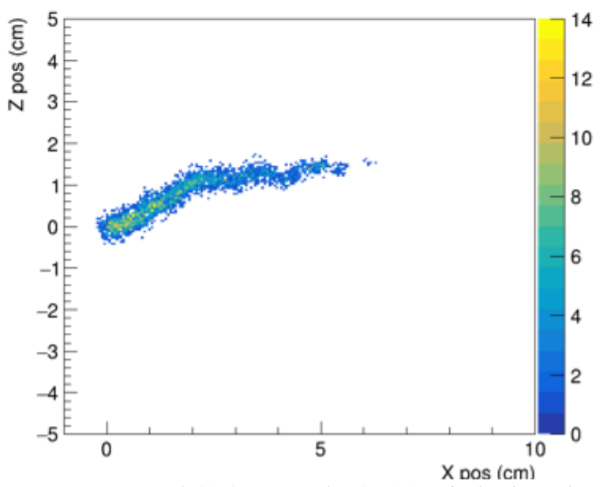
\includegraphics[width=0.5\textwidth]{../figures/Snipaste_2021-05-20_16-39-55.png}
    
      \caption{模拟的裂变碎片径迹在读出板上的信号}
      \label{fig-Test}
  \end{figure}
\end{frame}



\begin{frame}[t]
  \frametitle{深度学习人工神经网络的优点}
  利用\textcolor{red}{机器学习}进行气体探测器径迹重建的算法研究

  $\linebreak$
  $\linebreak$

  深度学习人工神经网络的优点:
  \begin{itemize}
    \item 能够近似模拟任何数学函数。
    \item 人工神经网络对非线性数据具有最好的甄别效果。
    \item 易于实现。
    \end{itemize}

\end{frame}








\section{基于裂变时间投影室的径迹重建}


% 第二章从模拟计算产生的 $^{235}$U 裂变碎片事件数据出发。使用 fortran 的 fissionlib 计算 1 MeV 中子轰击 $^{235}$U 后的产物分布,共生成 200000 例事件。
% 之后统计 200000 例裂变事件中的核素,使用 SRIM 生成每一个核素的重离子能损表。
% 最后使用 Garfield++ 调用 SRIM 的重离子能损表估算每一个裂变碎片在时间投影室内的径迹信息,完成裂变碎片的在时间投影室内的二维重建和三维径迹重建。


% 本章从使用 fissionlib 模拟 1 MeV 中子轰击 $^{235}$U 模拟生成的 200000 个裂变事件出发,借助 Garfield++(及其依赖的 Geant4 和 ROOT)和 Srim,模拟了裂变时间投影室以及裂变碎片在时间投影室室腔内的漂移,进而产生径迹信息。径迹信息包含电子在读出板上的坐标以及电子到达读出板上的时间等信息。
% 借助这些径迹信息以及利用 Garfield++ 计算出的漂移速度,完成了径迹的二维重建和三维重建。





\section{基于人工神经网络的裂变碎片分类模型}




\section{总结展望}




\end{document}